 
The depreciated value of an item refers to the assessed value of an item that has lost value due to wear and tear.  If an item is losing about $10\%$ of its prior year's value each year, which of the following graphs could model the depreciated value of an item as a function of time?
\\\\


\ifsat
	\begin{enumerate}[label=\Alph*)]
		\item 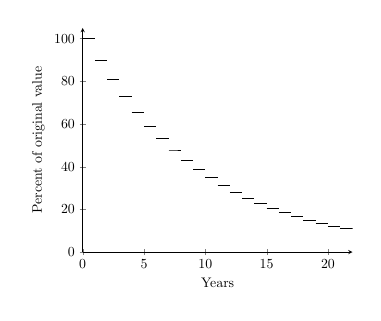
\begin{tikzpicture}[scale=0.5]\begin{axis}[axis lines=left, xtick={0,5,...,20}, ytick={0,20,...,100},xmin=0,xmax=22,ymin=0,ymax=105, ylabel={Percent of original value},xlabel={Years}]
 \foreach \i in {0,1,...,21}
 \addplot[domain=\i:\i+1,samples=3]{100*.9^\i};;
 \end{axis}\end{tikzpicture} 
		\item 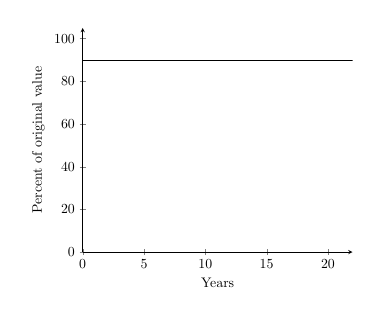
\begin{tikzpicture}[scale=0.5]\begin{axis}[axis lines=left, xtick={0,5,...,20}, ytick={0,20,...,100},xmin=0,xmax=22,ymin=0,ymax=105, ylabel={Percent of original value},xlabel={Years}]
 \addplot[samples=3,domain=0:22]{90};
 \end{axis}\end{tikzpicture}\\\\ 
		\item 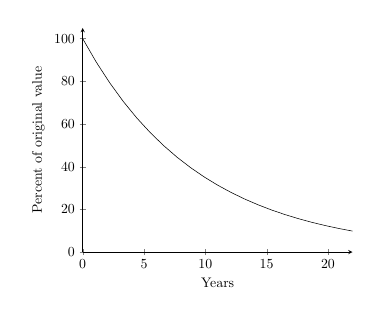
\begin{tikzpicture}[scale=0.5]\begin{axis}[axis lines=left, xtick={0,5,...,20}, ytick={0,20,...,100},xmin=0,xmax=22,ymin=0,ymax=105, ylabel={Percent of original value},xlabel={Years}]
 \addplot[samples=21,domain=0:22]{100*.9^x};
 \end{axis}\end{tikzpicture} % 
		\item 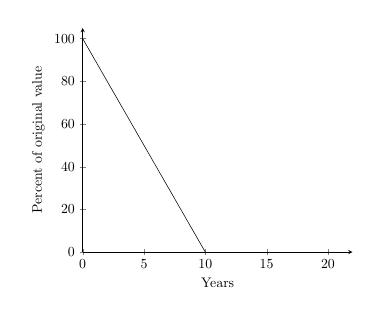
\begin{tikzpicture}[scale=0.5]\begin{axis}[axis lines=left, xtick={0,5,...,20}, ytick={0,20,...,100},xmin=0,xmax=22,ymin=0,ymax=105, ylabel={Percent of original value},xlabel={Years}]
 \addplot[samples=3,domain=0:22]{100-10*x};
 \end{axis}\end{tikzpicture} 
	\end{enumerate}
\else
\fi

\ifacteven
	\begin{enumerate}[label=\textbf{\Alph*.},itemsep=\fill,align=left]
		\setcounter{enumii}{5}
		\item 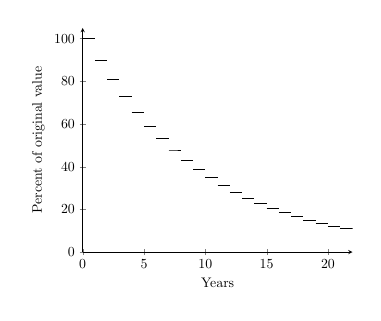
\begin{tikzpicture}[scale=0.5]\begin{axis}[axis lines=left, xtick={0,5,...,20}, ytick={0,20,...,100},xmin=0,xmax=22,ymin=0,ymax=105, ylabel={Percent of original value},xlabel={Years}]
 \foreach \i in {0,1,...,21}
 \addplot[domain=\i:\i+1,samples=3]{100*.9^\i};;
 \end{axis}\end{tikzpicture} 
		\item 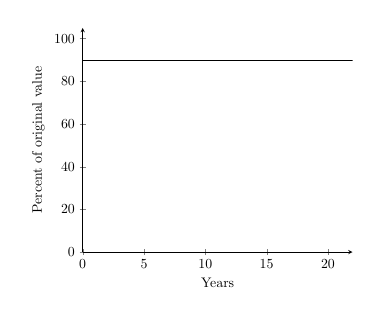
\begin{tikzpicture}[scale=0.5]\begin{axis}[axis lines=left, xtick={0,5,...,20}, ytick={0,20,...,100},xmin=0,xmax=22,ymin=0,ymax=105, ylabel={Percent of original value},xlabel={Years}]
 \addplot[samples=3,domain=0:22]{90};
 \end{axis}\end{tikzpicture}\\\\ 
		\item 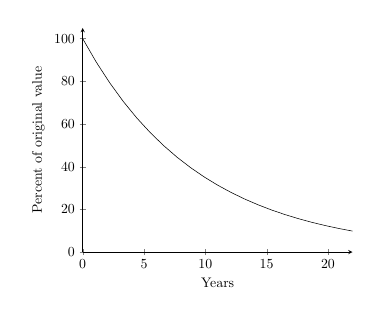
\begin{tikzpicture}[scale=0.5]\begin{axis}[axis lines=left, xtick={0,5,...,20}, ytick={0,20,...,100},xmin=0,xmax=22,ymin=0,ymax=105, ylabel={Percent of original value},xlabel={Years}]
 \addplot[samples=21,domain=0:22]{100*.9^x};
 \end{axis}\end{tikzpicture} % 
		\addtocounter{enumii}{1}
		\item 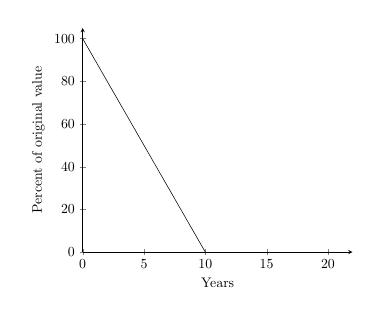
\begin{tikzpicture}[scale=0.5]\begin{axis}[axis lines=left, xtick={0,5,...,20}, ytick={0,20,...,100},xmin=0,xmax=22,ymin=0,ymax=105, ylabel={Percent of original value},xlabel={Years}]
 \addplot[samples=3,domain=0:22]{100-10*x};
 \end{axis}\end{tikzpicture} 
		\item None of these. 
	\end{enumerate}
\else
\fi

\ifactodd
	\begin{enumerate}[label=\textbf{\Alph*.},itemsep=\fill,align=left]
		\item 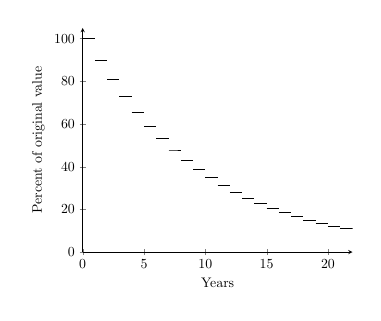
\begin{tikzpicture}[scale=0.5]\begin{axis}[axis lines=left, xtick={0,5,...,20}, ytick={0,20,...,100},xmin=0,xmax=22,ymin=0,ymax=105, ylabel={Percent of original value},xlabel={Years}]
 \foreach \i in {0,1,...,21}
 \addplot[domain=\i:\i+1,samples=3]{100*.9^\i};;
 \end{axis}\end{tikzpicture} 
		\item 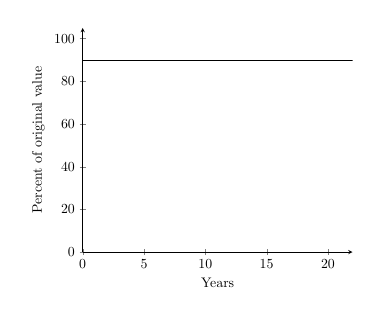
\begin{tikzpicture}[scale=0.5]\begin{axis}[axis lines=left, xtick={0,5,...,20}, ytick={0,20,...,100},xmin=0,xmax=22,ymin=0,ymax=105, ylabel={Percent of original value},xlabel={Years}]
 \addplot[samples=3,domain=0:22]{90};
 \end{axis}\end{tikzpicture}\\\\ 
		\item 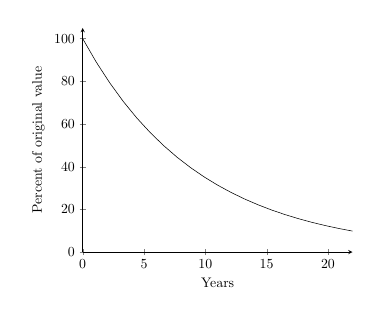
\begin{tikzpicture}[scale=0.5]\begin{axis}[axis lines=left, xtick={0,5,...,20}, ytick={0,20,...,100},xmin=0,xmax=22,ymin=0,ymax=105, ylabel={Percent of original value},xlabel={Years}]
 \addplot[samples=21,domain=0:22]{100*.9^x};
 \end{axis}\end{tikzpicture} % 
		\item 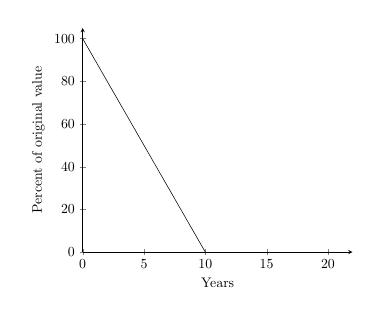
\begin{tikzpicture}[scale=0.5]\begin{axis}[axis lines=left, xtick={0,5,...,20}, ytick={0,20,...,100},xmin=0,xmax=22,ymin=0,ymax=105, ylabel={Percent of original value},xlabel={Years}]
 \addplot[samples=3,domain=0:22]{100-10*x};
 \end{axis}\end{tikzpicture} 
		\item None of these. 
	\end{enumerate}
\else
\fi

\ifgridin
 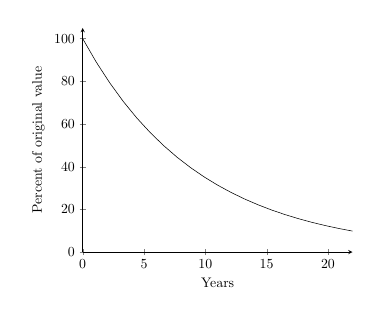
\begin{tikzpicture}[scale=0.5]\begin{axis}[axis lines=left, xtick={0,5,...,20}, ytick={0,20,...,100},xmin=0,xmax=22,ymin=0,ymax=105, ylabel={Percent of original value},xlabel={Years}]
 \addplot[samples=21,domain=0:22]{100*.9^x};
 \end{axis}\end{tikzpicture} % 
		
\else
\fi

